\section{Casi d'uso}
\label{sez:use}

In questa sezione vedremo come vengono modellati i protocolli tramite diagrammi UML, come il tool di conversione utilizza i file .xmi per arrivare a generare dei file da dare in input a VerifPal e quali sono le risposte dei risultati dell'analisi.\\
I protocolli utilizzati come esempio sono il protocollo di Needham e Schroeder a chiave simmetrica, il protocollo ARP e il crittosistema RSA.\\
\subsection{Needham Schroeder Symmetric Key}

In questa sezione vedremo come è possibile modellare attraverso i diagrammi object diagram dello standard UML il protocollo di sicurezza a chiave simmetrica proposto da Needham e Schroeder:
\begin{lstlisting}[mathescape]
    1. $A \rightarrow S : A, B, N_a$
    2. $S \rightarrow A : \{N_a, K_{ab}, B, \{K_{ab}, A\}_{K_{bs}}\}_{K_{as}}$
    3. $A \rightarrow B : \{K_{ab}, A\}_{K_{bs}}$
    4. $B \rightarrow A : \{N_b\}_{K_{as}}$
    5. $A \rightarrow B : \{N_b-1\}_{K_{as}}$
\end{lstlisting} 

\noindent Nelle Figure seguenti avremo i seguenti partecipanti al protocollo: l'agente \texttt{Initiator} che vuole iniziare la comunicazione con l'agente \texttt{Recipient} e richiede la password per la comunicazione al server \texttt{S}.\\
Inoltre la chiave simmetrica viene rappresentata in questo modo \texttt{SK($a$,$b$)}, dove $a$ e $b$ indicano l'identità degli agenti proprietari della chiave.\\
\newpage
\begin{figure}[h!] 
    \centering 
    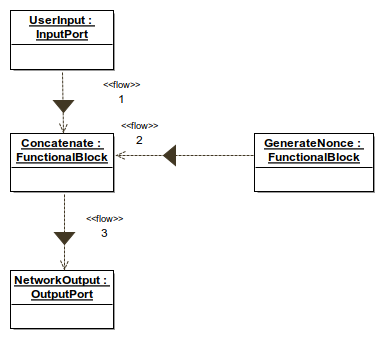
\includegraphics[scale=0.6]{../img/NSSK/First_message(toServer)_Object_diagram.png} 
    \begin{lstlisting}[frame=single, mathescape, basicstyle=\footnotesize]
        1. $<i.name, r.name>$
        2. $<i.nonce>$
        3. $<i.name, r.name, i.nonce>$
    \end{lstlisting}
    \caption{$A \rightarrow B : A, B, N_a$} 
\end{figure}
\noindent Nell'oggetto UserInput il sistema che andrà ad implementare il protocollo riceve il nome ($r.name$) dell'agente \texttt{Recipient}, l'oggetto GenerateNonce genera un nuovo Nonce e l'oggetto Concatenate prepara il pacchetto da mandare al server \texttt{S} attraverso l'oggetto NetworkOPort, composto da $i.name, r.name, i.nonce$, ovvero dai nomi dei partecipanti al protocollo e il nonce per assicurarsi che la comunicazione sia fresh.
\newpage
\begin{figure}[h!] 
    \centering 
    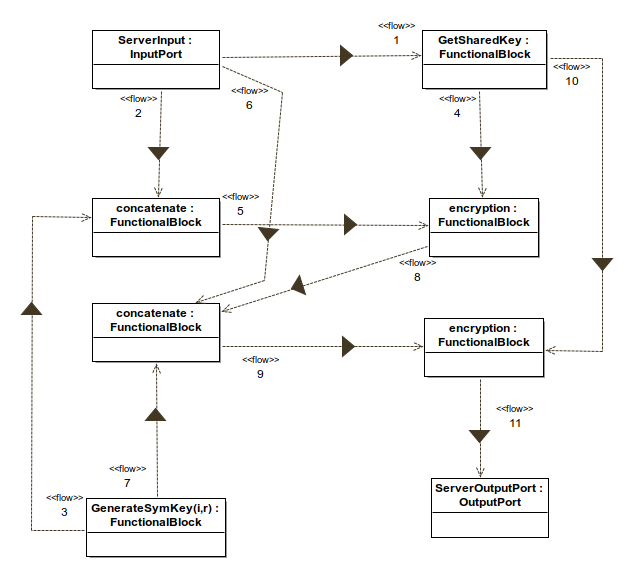
\includegraphics[scale=0.5]{../img/NSSK/Second_Message(fromServer).png} 
    \begin{lstlisting}[frame=single, mathescape, basicstyle=\footnotesize]
        1. $<i.name,r.name>$
        2. $<i.name>$
        3. $<SK(i,r)>$
        4. $<SK(s,r)>$
        5. $<i.name, SK(i,r)>$
        6. $<r.name, i.nonce>$
        7. $<SK(i,r)>$
        8. $<\{i.name; SK(i,r)\}\_SK(r,s)>$
        9. $<i.nonce, r.name, SK(i,r), \{i.name,SymKey(i,r)\}\_SK(r,s)\}>$
        10. $<SK(s,r)>$
        11. $<\{i.nonce, r.name, SK(i,r), \{i.name,SK(i,r)\}\_SK(rs)\}\}\_SK(i,s)>$
    \end{lstlisting}
    \caption{$S \rightarrow A : \{N_a, K_{ab}, B, \{K_{ab}, A\}_{K_{bs}}\}_{K_{as}}$} 
\end{figure}
\noindent Una volta ricevuto il pacchetto, il server \texttt{S} provvede alla generazione della chiave simmetrica (\texttt{SK($i$,$r$)}) per la comunicazione tra \texttt{Initiator} e \texttt{Recipient} utilizzando l'oggetto GenerateSymKey($i$,$r$), passando a quest'ultimo i nomi $i.name, r.name$ dei partecipanti.\\ 
A questo punto, fornendo sempre come input i nomi dei partecipanti all'oggetto GetSharedKey, ottiene le chiavi simmetriche precedentemente condivise tra lui e ogni agente partecipante (\texttt{SK($i$,$s$)} e \texttt{SK($r$,$s$)}).\\ 
La chiave \texttt{SK($r$,$s$)} verrà utilizzata dall'oggetto encryption dopo aver preparato con l'oggetto Concatenate il pacchetto per l'agente \texttt{Recipient}, questo pacchetto a sua volta verrà inserito da un altro oggetto Concatenate nel pacchetto per l'agente \texttt{Initiator} e il tutto verrà cifrato da un altro oggetto encryption con la chiave \texttt{SK($i$,$s$)}. Il pacchetto risultante da queste operazioni verrà spedito all'agente \texttt{Initiator} attraverso l'oggetto ServerOutputPort.\\

\begin{figure}[h!] 
    \centering 
    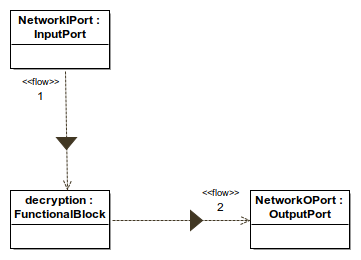
\includegraphics[scale=0.6]{../img/NSSK/FirstMessage.png} 
    \begin{lstlisting}[frame=single, mathescape, basicstyle=\footnotesize]
        1. $<\{i.nonce, r.name, SK(i,r), \{i.name,SK(i,r)\}\_SK(r,s)\}\_SK(i,s)>$
        2. $<\{i.name,SK(i,r)\}\_SK(r,s)>$
    \end{lstlisting}
    \caption{$A \rightarrow B : \{K_{ab}, A\}_{K_{bs}}$} 
\end{figure}
\noindent L'agente \texttt{Initiator} riceve il pacchetto attraverso l'oggetto NetworkIPort e utilizza l'oggetto di decryption con la chiave simmetrica \texttt{SK($i$,$s$)} per estrarre il pacchetto da inoltrare all'agente \texttt{Recipient} attraverso l'oggetto NetworkOPort.\\
\begin{figure}[h!] 
    \centering 
    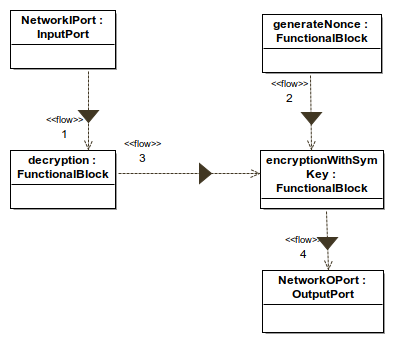
\includegraphics[scale=0.59]{../img/NSSK/SecondMessage.png} 
    \begin{lstlisting}[frame=single, mathescape, basicstyle=\footnotesize]
        1. $<\{i.name,SK(i,r)\}\_SK(r,s)>$
        2. $<r.nonce>$
        3. $<SK(i,s)>$
        4. $<\{r.nonce\}\_SK(i,r)>$
    \end{lstlisting}
    \caption{$B \rightarrow A : \{N_b\}_{K_{as}}$} 
\end{figure}
\newpage
\noindent L'agente \texttt{Recipient} riceve il pacchetto attraverso l'oggetto NetworkIPort, lo decifra con l'oggetto decryption utilizzando la chiave \texttt{SK($r$,$s$)} ed estrae la chiave \texttt{SK($i$,$r$)}.\\ 
\texttt{SK($i$,$r$)} verrà utilizzata dall'oggetto encryptionWithSymKey per cifrare un nuovo pacchetto contenente il Nonce generato dall'oggetto generateNonce.\\ 
Infine l'agente \texttt{Recipient} spedisce il pacchetto all'agente \texttt{Initiator} utilizzando l'oggetto NetworkOPort.\\
\begin{figure}[h!] 
    \centering 
    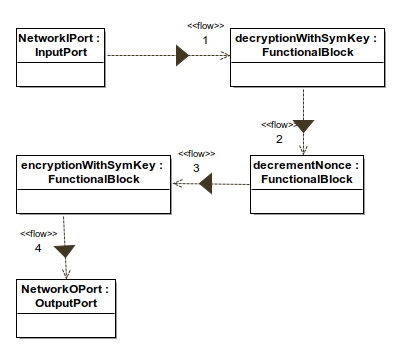
\includegraphics[scale=0.6]{../img/NSSK/ThirdMessage.png} 
    \begin{lstlisting}[frame=single, mathescape, basicstyle=\footnotesize]
        1. $<{r.nonce}\_SK(i,r)>$
        2. $<r.nonce>$
        3. $<r.nonce-1>$
        4. $<\{r.nonce-1\}\_SK(i,r)>$
    \end{lstlisting}
    \caption{$A \rightarrow B : \{N_b-1\}_{K_{as}}$} 
\end{figure}\\
\noindent Nell'ultima fase del protocollo, l'agente \texttt{Initiator} riceve dall'oggetto NetworkIPort il pacchetto contenente il Nonce, lo decifra con l'oggetto decryptionWithSymKey utilizzando la chiave \texttt{SK($i$,$r$)}, utilizza l'oggetto decrementNonce per sottrarre 1 al Nonce inviato dall'agente \texttt{Recipient} e cifra il risultato con l'oggetto encryptionWithSymKey utilizzando la chiave \texttt{SK($i$,$r$)}.\\
Il pacchetto risultante viene spedito all'agente \texttt{Recipient} attraverso l'oggetto NetworkOPort.\\

\newpage
\subsubsection*{Tool di verifica}
Dopo aver modellato il protocollo ed estratto il file .xmi visibile nel Listing \ref{lst:ns1}\footnote{\label{note:a}Listing in Appendice \ref{app:ns}}, si utilizza il tool di conversione per ottenere il file delle strutture Listing \ref{lst:ns2}\textsuperscript{\ref{note:a}}.\\
Sempre con il tool di conversione ricaviamo il seguente file da utilizzare come input a VerifPal:

\lstinputlisting[label={lst:nssk.vp},caption={File nssk.vp},language=vp, breaklines= true]{../code/verifpal/nssk.vp}

\noindent In questo esempio vengono verificate la confidenzialità della chiave \textbf{k\_ir}, la confidenzialità del Nonce \textbf{n\_r\_minus\_one} e l'autenticazione dell'ultimo pacchetto del protocollo.\\
Nel Listing \ref{lst:ns3}\footnote{Listing in Appendice \ref{app:ns}} troviamo il risultato dell'analisi.\\
Come dimostrato da Denning-Sacco in \cite{DS81} il protocollo è soggetto ad attacchi di tipo reply attack, se l'attaccante viene a conoscenza della chiave condivisa tra i due principal.\\
In questo modello l'attaccante in qualche modo riesce ad ottenere la chiave e di conseguenza i risultati della verifica diranno che la chiave non è confidenziale, come non è confidenziale il Nonce \textbf{n\_r\_minus\_one}, oltre al fatto che può essere lo stesso attaccante ad inviare il pacchetto \textbf{e\_n\_r\_minus\_one} al principal \texttt{Recipient} fingendosi il principal Initiator, violando l'autenticazione.\\
Per completezza in Appendice \ref{app:ns} vengono riportate la modellazione del protocollo in Applied Pi Calculus nel Listing \ref{lst:ns4} e i risultati ottenuti con ProVerif nel Listing \ref{lst:ns5}, i quali rispecchiano i risultati ottenuti con VerifPal.

\subsubsection*{Osservazioni}
L'esecuzione del modello di questo protocollo consiste in una sola sessione dove l'attaccante è a conoscenza della chiave simmetrica tra i due principal, questo definisce uno scenario ben specifico infatti non è sempre vero che l'attaccante riesca ad ottenere la chiave simmetrica.\\
Con questa premessa si capisce come l'utilizzatore del tool per la verifica dovrebbe avere ben chiaro lo scenario in cui modellare il protocollo e allo stesso tempo dovrebbe avere almeno l'intuizione per capire sotto quali condizioni il protocollo può essere violato, per poterlo testare in diversi scenari.\\
Facendo vari tipi di verifiche sul protocollo è infatti emerso un limite dei verificatori automatici, ovvero il fatto di dover modellare il protocollo in uno specifico scenario per verificare la presenza di un determinato tipo di attacco, eventualmente già noto.\\ 
Per diversificare gli scenari, l'utilizzatore del tool può aumentare il numero di sessioni del protocollo, oppure fornire ad un certo punto dell'esecuzione del protocollo delle informazioni all'attaccante, come abbiamo visto in questo caso.\\
Queste tecniche consentono al tool di verifica di fornire delle risposte valide ai quesiti, evitando la non terminazione o risposte del tipo ``Non lo so''. 

\newpage
\subsection{Address Resolution Protocol}
Lo scopo del protocollo ARP descritto in \cite{RFC0826} e in \cite{RFC5227} è quello di eseguire una mappatura tra indirizzo IP e indirizzo MAC di una macchina all'interno di una rete locale Ethernet.\\
La notazione seguente utilizzata nei pacchetti è ripresa da \cite{RFC0826}:
\begin{lstlisting}
    ar$hrd: Hardware address space 
    ar$pro: Protocol address space
    ar$hln: byte length of each hardware address
    ar$pln: byte length of each protocol address
    ar$op:  opcode (request | reply)
    ar$sha: Hardware address of sender 
    ar$spa: Protocol address of sender 
    ar$tha: Hardware address of target
    ar$tpa: Protocol address of target
\end{lstlisting}
In Figura \ref{fig:ARP} vediamo come si modella il protocollo ARP.\\
Una macchina, appena connessa alla rete o accesa, si mette subito in ascolto con l'oggetto ANNOUNCE\_WAIT e, allo stesso tempo, utilizza gli oggetti getIPAddress per generare un indirizzo IP sul quale essere contattata, getProtocolType e getMACAddress  per ricavare informazioni sul tipo di protocollo ethernet da utilizzare e l'indirizzo MAC della sua scheda di rete.\\
A questo punto utilizza queste informazioni per creare attraverso l'oggetto createProbePackage un pacchetto da inviare in broadcast a tutte le macchine della rete.\\
Successivamente attende un tempo predefinito attraverso l'oggetto PROBE\_WAIT, prima di spedire il pacchetto attraverso l'oggetto EthernetOUT e ritornare nello stato di ANNOUNCE\_WAIT.\\
Se nell'arco di un tempo predefinito non arriva nessun pacchetto dall'oggetto EthernetIN, procede con la conferma dell'indirizzo IP attraverso la creazione di un nuovo pacchetto con l'oggetto createAnnouncePackage, il quale verrà sempre spedito in broadcast attraverso l'oggetto EthernetOUT.\\
Se invece riceve un pacchetto dall'oggetto EthernetIN, ricomincia generando un nuovo indirizzo IP.\\
\begin{figure}[h!] 
    \centering 
    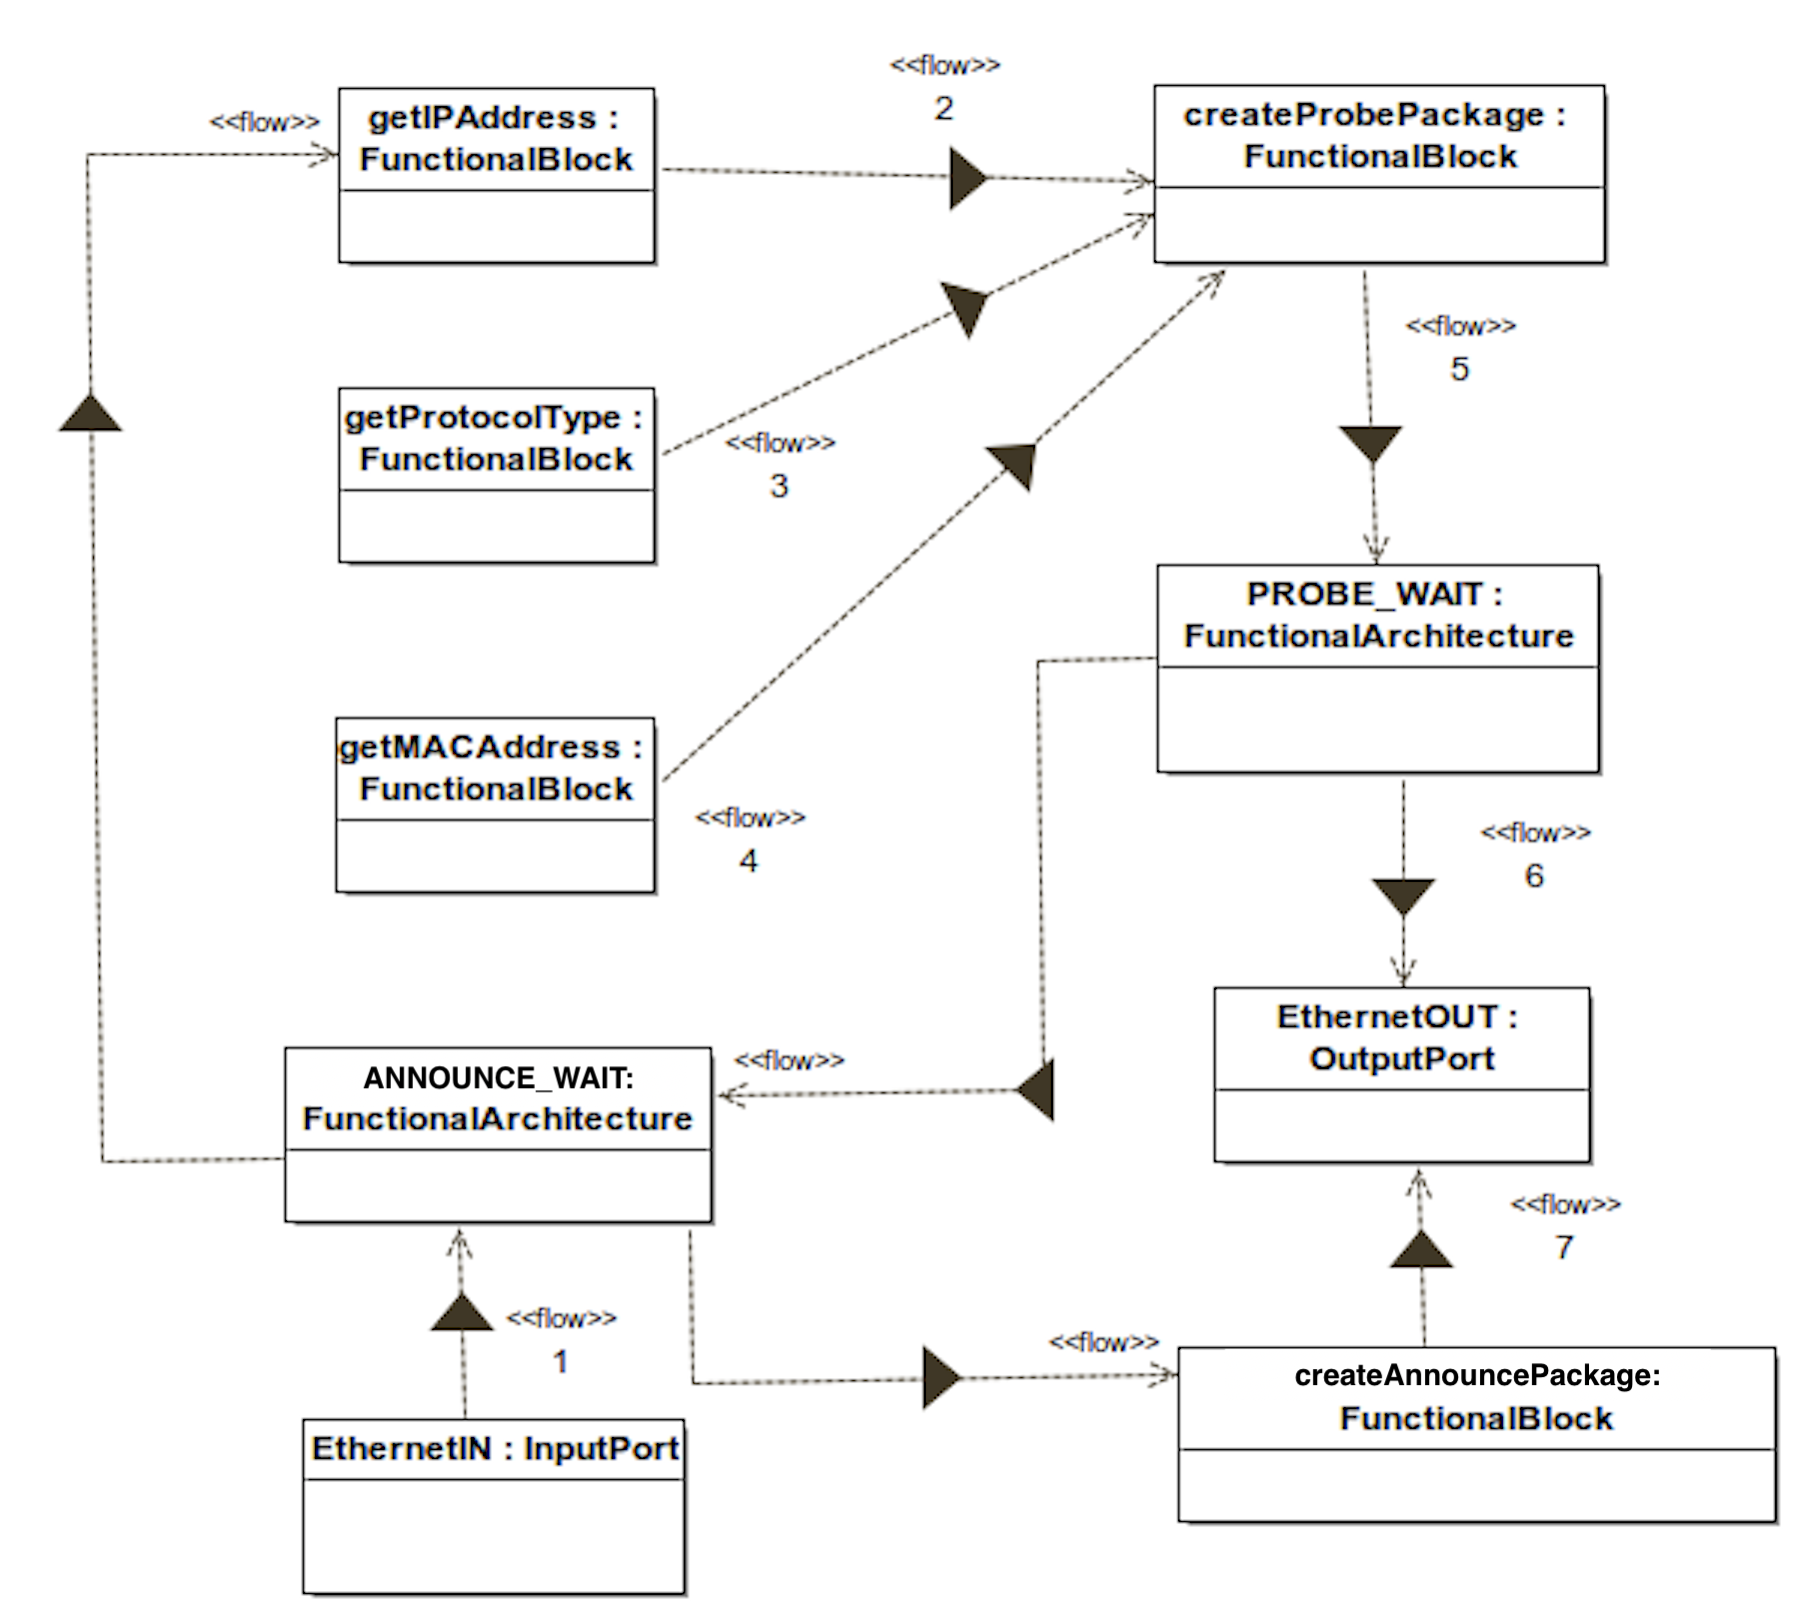
\includegraphics[scale=0.35]{../img/ARP/ARP.png}
    \begin{lstlisting}[frame=single, mathescape, basicstyle=\footnotesize]
1. $<\{as\$hrd, ar\$pro, ar\$hln, ar\$pln, reply, ar\$sha, ar\$spa, ar\$tha, ar\$tpa\}>$
2. $<ip>$
3. $<ar\$spa>$
4. $<ar\$sha>$
5. $<\{as\$hrd, ar\$pro, ar\$hln, ar\$pln, request, ar\$sha, 0.0.0.0, 00:00:00:00:00:00, ip\}>$
6. $<\{as\$hrd, ar\$pro, ar\$hln, ar\$pln, request, ar\$sha, 0.0.0.0, 00:00:00:00:00:00, ip\}>$
7. $<\{as\$hrd, ar\$pro, ar\$hln, ar\$pln, request, ar\$sha, ip, 00:00:00:00:00:00, ip\}>$
    \end{lstlisting}
    \caption{Modellazione del protocollo ARP} 
    \label{fig:ARP}
\end{figure}
\newpage
\begin{figure}[h!] 
    \centering 
    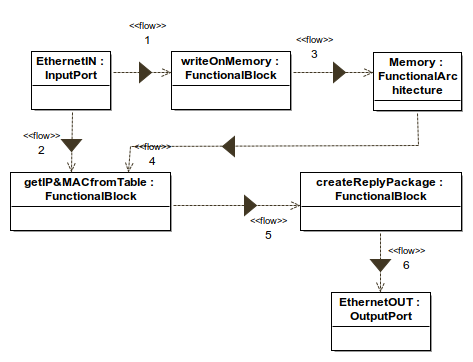
\includegraphics[scale=0.5]{../img/ARP/ARP_Reply_Object_diagram.png} 
\begin{lstlisting}[frame=single, mathescape, basicstyle=\footnotesize]
1. $<\{as\$hrd, ar\$pro, ar\$hln, ar\$pln, request, ar\$sha, ip, 00:00:00:00:00:00, ip\}>$
2. $<\{as\$hrd, ar\$pro, ar\$hln, ar\$pln, request, ar\$sha, 0.0.0.0, 00:00:00:00:00:00, ip\}>$
3. $<ar\$sha, ip>$
4. $<ar\$tha, ar\$tpa>$
5. $<ar\$tha, ar\$tpa>$
6. $<\{as\$hrd, ar\$pro, ar\$hln, ar\$pln, reply, ar\$sha, ar\$spa, ar\$tha, ar\$tpa\}>$
\end{lstlisting}
    \caption{Modellazione del blocco di ARP Reply} 
    \label{fig:ARP2}
\end{figure}
\noindent Nel caso in cui una macchina della rete riceva un pacchetto dall'oggetto EthernetIN (Figura \ref{fig:ARP2}), la prima cosa che fa è verificare se si tratta di un pacchetto di probe oppure di un pacchetto di announce.\\
Nel primo caso va a verificare con l'oggetto Memory se nell'ARP cache è già presente quell'indirizzo IP, assegnato ad un indirizzo MAC, che non corrisponde a quello del sender del pacchetto.\\ 
Se vi è una corrispondenza tra l'indirizzo ip del sender del pacchetto ed uno già presente nell'ARP cache, allora l'oggetto getIP\&MACFromTable riceve in input le informazioni dalla ARP cache per generare un nuovo pacchetto attraverso l'oggetto createReplyPackage, con il quale rispondere in unicast al sender attraverso l'oggetto EthernetOut, altrimenti non fa nulla.\\
Nel caso in cui si tratti di un pacchetto di announce allora l'oggetto writeOnMemory si occuperà di salvare nella ARP cache la mappatura tra l'indirizzo IP e MAC del sender.\\

\subsubsection*{Tool di verifica}
Dopo aver modellato il protocollo ed estratto il file .xmi visibile nel Listing \ref{lst:arp1}\footnote{\label{note:b}Listing in Appendice \ref{app:arp}}, si utilizza il tool di conversione per ottenere il file delle strutture Listing \ref{lst:arp2}\textsuperscript{\ref{note:b}}.\\
Per quanto già detto precedentemente, essendo il protocollo ARP suddivisibile in più scenari come l'invio del pacchetto di probe seguito dall'invio del pacchetto di announce oppure l'invio del pacchetto di probe seguito dall'invio del pacchetto di reply, una volta generato il template completo deve essere l'utilizzatore a suddividere i vari scenari per poi sottoporli alla verifica con Verifpal.\\
Per dividere i due scenari, l'utilizzatore deve generare due file da utilizzare come input in VerifPal, per fare questo è sufficiente copiare il template completo ed andare a cancellare le righe di generazione e invio del pacchetto di announce quando si vuole rappresentare lo scenario dell'invio del pacchetto di probe seguito dall'invio del pacchetto di reply, allo stesso modo per rappresentare lo scenario di invio di un pacchetto di probe seguito da un pacchetto di announce, l'utilizzatore non deve fare altro che cancellare le righe contenenti la creazione e l'invio del pacchetto di reply.
\newpage
\lstinputlisting[label={lst:arp_annunce.vp},caption={File arp\_announce.vp},language=vp, breaklines= true]{../code/verifpal/arp_annunce.vp}
\newpage
\lstinputlisting[label={lst:arp_reply.vp},caption={File arp\_reply.vp},language=vp, breaklines= true]{../code/verifpal/arp_reply.vp}

\noindent Come ben noto, il protocollo ARP è un protocollo di rete che non si occupa dell'integrità dei pacchetti ed è vulnerabile ad un attacco chiamato ARP Poisoning, questo attacco consiste in un attacco del tipo Man In The Middle, dove l'attaccante modifica i pacchetti che attraversano la rete per andare a modificare con valori inesatti le ARP cache delle macchine connesse.\\
L'obiettivo della modifica della mappatura tra indirizzo MAC e indirizzo IP può essere attuare un Denial Of Service oppure fingersi una determinata macchina.\\
Dato l'utilizzo dell'attaccante attivo da parte del tool VerifPal, come possiamo vedere dai Listing \ref{lst:arp3}-\ref{lst:arp4}\footnote{Listing in Appendice \ref{app:arp}}, l'attaccante riesce a violare sia la confidenzialità che l'integrità dei pacchetti, di conseguenza riesce ad attuare l'attacco di tipo ARP Poisoning.\\
Per confermare quanto appena detto in Appendice \ref{app:arp} vengono riportate la modellazione dello scenario di invio di un pacchetto di probe descritto in Applied Pi Calculus nel Listing \ref{lst:arp5} e il risultato della verifica svolta con ProVerif nel Listing \ref{lst:arp6}.\\ 

\subsection{Crittosistema RSA}
Nel 1978 in \cite{RSA78} Rivest, Shamir e Adleman hanno proposto un crittosistema per la cifratura e la firma dei messaggi basato sulla crittografia asimmetrica.\\
Come vedremo nelle Figure successive il crittosistema si basa su tre funzioni principali: funzione di generazione delle chiavi, funzione di encryption e funzione di decryption.\\
Nella modellazione UML ogni oggetto rappresenta le funzioni matematiche utilizzate dalle tre funzioni.\\ 
L'oggetto Memory viene utilizzato dalla funzione di generazione delle chiavi per salvare le informazioni riguardo la chiave pubblica e la chiave privata necessarie alle funzioni di encryption e decryption.\\  

\begin{figure}[h!] 
    \centering 
    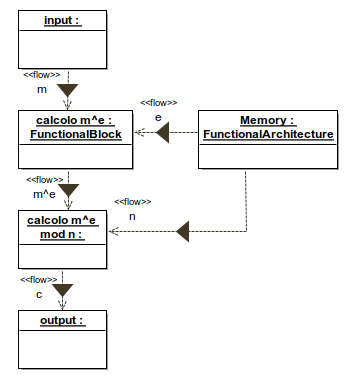
\includegraphics[scale=0.5]{../img/RSA/Encryption_Object_diagram.png} 
    \caption{Funzione di encryption} 
\end{figure}

\begin{figure}[h!] 
    \centering 
    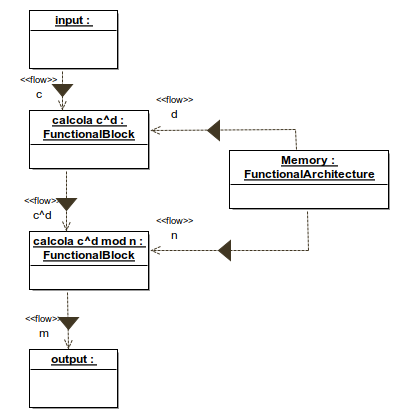
\includegraphics[scale=0.5]{../img/RSA/Decryption_Object_diagram.png} 
    \caption{Funzione di decryption} 
\end{figure}
\begin{figure}[h!] 
    \centering 
    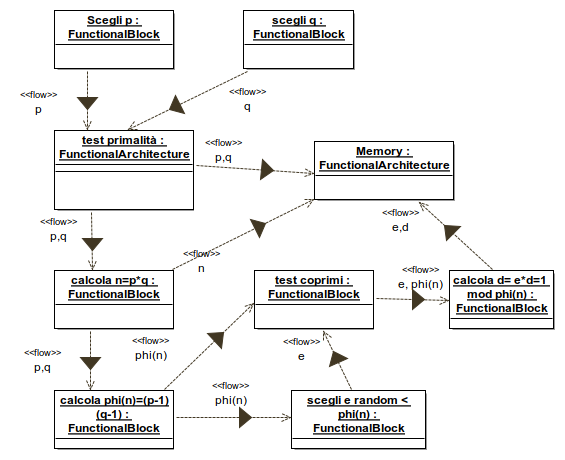
\includegraphics[scale=0.5]{../img/RSA/Key_Generation_Object_diagram.png} 
    \caption{Generazione delle chiavi} 
\end{figure}

\clearpage
\subsubsection*{Tool di verifica}
A seguito della modellazione UML del crittosistema RSA è possibile utilizzare il file .xmi estratto, visibile nel Listing \ref{lst:rsa1}\footnote{\label{note:c}Listing presentati in Appendice \ref{app:rsa}} per generare il file delle strutture Listing \ref{lst:rsa2}\textsuperscript{\ref{note:c}}.\\
In questo caso ci troviamo però in un caso particolare per il tool di conversione perch\'e il tool di analisi VerifPal utilizza un attaccante del modello Dolev-Yao, il quale non è in grado di rompere le primitive crittografiche, ed inoltre lo stesso VerifPal ci fornisce le primitive di encryption e decryption senza dover implementare nulla.\\
Per questo motivo deve essere l'utilizzatore a modellare il file da dare in input al tool di verifica a mano, andando ad ipotizzare uno scenario in cui viene utilizzato RSA:
\lstinputlisting[label={lst:nssk.vp},caption={File nssk.vp},language=vp, breaklines= true]{../code/verifpal/rsa.vp}
Come vediamo nel Listing \ref{lst:rsa3}\footnote{\label{note:d}Listing presentati in Appendice \ref{app:rsa}} il risultato della verifica sulla confidenzialità del messaggio \textbf{m\_b} viene preservata, questo perch\'e è il risultato della decryption con la chiave privata del principal e non è mai transitato in chiaro nella rete, ma viene trovato un problema di autenticazione per il messaggio \textbf{e\_2}, questo perch\'e per come è stato modellato il protocollo, l'attaccante può fingersi il secondo partecipante al protocollo andando a creare una coppia chiave pubblica-privata e inviare la sua chiave pubblica al posto di quella del reale partecipante.\\
La stessa situazione si verifica con la modellazione in Applied Pi Calculus (Listing \ref{lst:rsa4}\textsuperscript{\ref{note:d}}) come si può vedere dai risultati ottenuti con ProVerif (Listing \ref{lst:rsa5}\textsuperscript{\ref{note:d}}).\\
Ovviamente cambiando il tipo di scenario, ad esempio facendo in modo che le chiavi pubbliche siano certificate da una Public Key Infrastructure, i due tool di verifica automatica non rileveranno nessun tipo di problema riguardo autenticazione e confidenzialità.\\
Un metodo semplice di modellare questo nuovo scenario è quello di utilizzare una guardia sulle chiavi pubbliche scambiate dai principal, in modo che l'attaccante non possa n\'e leggerle, n\'e modificarle: 
\begin{lstlisting}[language=vp,mathescape]
    Alice -> Bob : [ga]
    Bob -> Alice : [gb]
\end{lstlisting}
\newpage
